\documentclass[10pt]{article}
\usepackage[margin=1in]{geometry}
\usepackage{graphicx}
\usepackage{booktabs}
\usepackage{amsmath}
\usepackage{listings}
\usepackage{xcolor}
\usepackage{hyperref}
\usepackage[font=small]{caption}

\lstset{basicstyle=\ttfamily\footnotesize, breaklines=true,
        keywordstyle=\color{blue}, commentstyle=\color{gray}, language=C++}

\title{A Fused STFT + Mel Filterbank CUDA Kernel:\\
       $3\times$ Faster Log-Mel Spectrograms than torchaudio}
\author{Nikhil Vincent}
\date{July 2026}

\begin{document}
\maketitle

\begin{abstract}
Log-mel spectrograms are the dominant input representation for audio machine
learning, yet the standard GPU implementation in torchaudio executes them as a
chain of ten kernel launches with intermediate results staged through global
memory. For the short clips typical of edge-audio inference (0.5--10\,s), the
pipeline is launch-latency-bound rather than compute-bound. We present a fused
CUDA kernel that combines magnitude computation, mel-filterbank projection,
and log scaling into a single launch, holding the power spectrum in shared
memory and exploiting the compact support of triangular mel filters to replace
the dense filterbank matmul with sparse per-filter dot products. On an NVIDIA
GB10, the fused pipeline computes a log-mel spectrogram of a 3.5\,s clip in
21.2\,\textmu s versus torchaudio's 60.8\,\textmu s---a $2.9\times$ speedup,
rising to $3.1\times$ on 0.5\,s and 10\,s clips---while matching torchaudio's
output to a maximum absolute error of $2\times10^{-5}$. Code:
\url{https://github.com/nikhilvincentv/cuda-mel-spectrogram}.
\end{abstract}

\section{Background}

The short-time Fourier transform splits a waveform $x[n]$ into overlapping
frames of length $N$ (hop $H$), applies a window $w[n]$, and computes for
frame $t$ and frequency bin $k$:
\begin{equation}
X[t,k] = \sum_{n=0}^{N-1} x[tH+n]\, w[n]\, e^{-2\pi i kn/N},
\qquad k = 0,\dots,N/2.
\end{equation}
The power spectrogram $P[t,k] = |X[t,k]|^2$ is projected onto $M$ mel-spaced
triangular filters, $\mathrm{mel}(f) = 2595\log_{10}(1+f/700)$ (HTK
convention), giving $S[t,m] = \sum_k B[m,k]\, P[t,k]$, followed by
$\log(S+\varepsilon)$. Each filter $B[m,\cdot]$ is nonzero only on a short
contiguous bin range---a fact the fused kernel exploits.

torchaudio's GPU path (\texttt{transforms.MelSpectrogram} + log) executes this
as ten CUDA kernels: padding, framing, windowing, cuFFT stages, magnitude,
a dense $(M \times K)$ filterbank matmul, and elementwise log, with the full
power spectrogram and pre-log mel spectrogram both materialized in DRAM.

\section{Implementation}

\textbf{Baseline (naive).} Our baseline mirrors torchaudio's structure but
already streamlines it to seven launches: a framing+window kernel (one block
per frame, coalesced), one batched cuFFT R2C plan covering all frames
(plan cached across calls, as torchaudio also does), a magnitude kernel, a
cuBLAS SGEMM for the mel projection, and a log kernel. Two intermediate
buffers (power spectrogram, pre-log mel) round-trip through global memory.

\textbf{Fused kernel.} The fused version replaces the last three stages
(magnitude, projection, log) with a single kernel, four launches total. One
thread block serves one frame:
\begin{enumerate}
  \item \emph{Phase 1:} 256 threads cooperatively compute $|X[t,k]|^2$ for the
        frame's $K = N/2{+}1$ bins, writing directly into shared memory. The
        power spectrum never reaches DRAM.
  \item \emph{Phase 2:} after \texttt{\_\_syncthreads()}, each thread owns one
        or more mel filters and accumulates a sparse dot product over only
        that filter's nonzero support, stored CSR-style as
        \texttt{(weights, offsets, start\_bin)} and read through
        \texttt{\_\_ldg}. It applies $\log(\cdot+\varepsilon)$ and writes one
        output float.
\end{enumerate}
The sparse layout reduces the projection from $O(MK)$ dense work to the sum of
filter support widths (about $2K$ total weights), and shared-memory reuse
means each power value is read by at most two filters at shared-memory rather
than DRAM latency.

\section{Results}

Benchmarks on an NVIDIA GB10 (DGX Spark, CUDA 13.0, PyTorch 2.12.1,
torchaudio 2.12.1): 20 warmup + 100 timed iterations, CUDA-event timing,
config sr=16\,kHz, $N{=}512$, $H{=}160$, $M{=}64$.

\begin{table}[h]\centering\small
\begin{tabular}{lrrrrr}
\toprule
clip & fused & naive & torchaudio GPU & librosa CPU & speedup \\
\midrule
0.5\,s & 20.0\,\textmu s & 28.9\,\textmu s & 62.1\,\textmu s & 336\,\textmu s & $3.10\times$ \\
1.0\,s & 20.4\,\textmu s & 29.1\,\textmu s & 61.7\,\textmu s & 401\,\textmu s & $3.02\times$ \\
3.5\,s & 21.2\,\textmu s & 30.0\,\textmu s & 60.8\,\textmu s & 781\,\textmu s & $2.87\times$ \\
10\,s  & 27.1\,\textmu s & 41.8\,\textmu s & 84.0\,\textmu s & 1735\,\textmu s & $3.10\times$ \\
\bottomrule
\end{tabular}
\caption{Mean latency per call (std $<$ 7\% in all cases). Speedup is fused
vs.\ torchaudio GPU.}
\end{table}

\begin{figure}[h]\centering
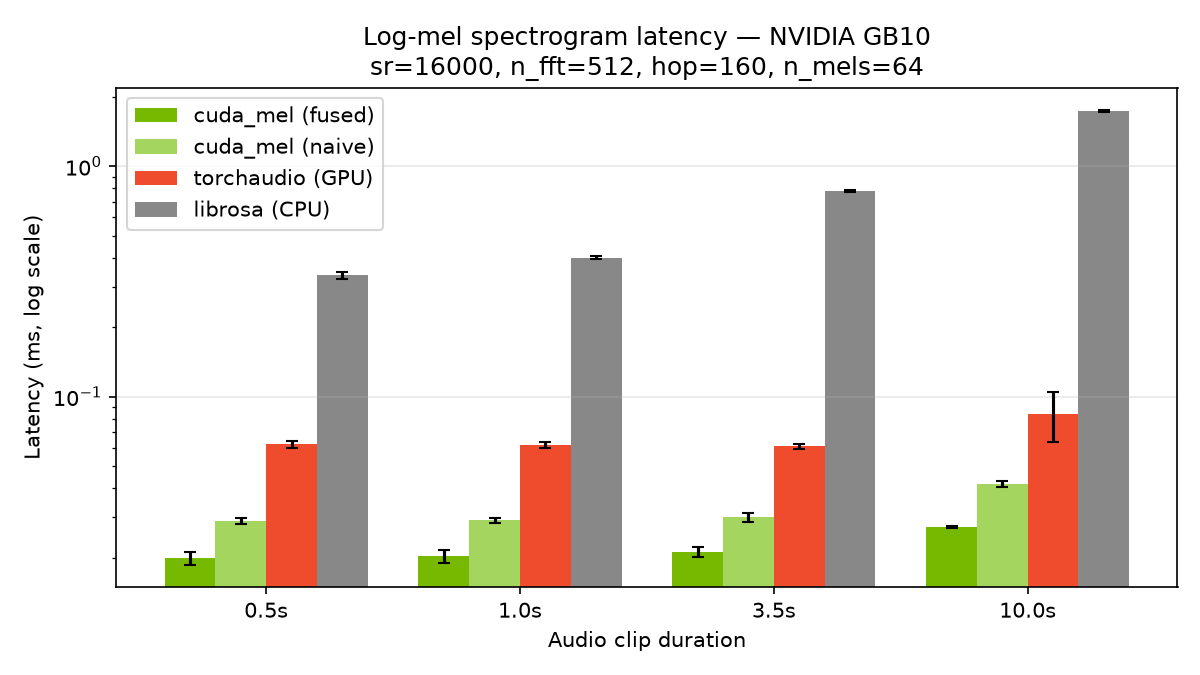
\includegraphics[width=0.78\textwidth]{../figures/latency_vs_duration.png}
\caption{Latency by implementation and clip length (log scale).}
\end{figure}

\textbf{Profiling.} Nsight Compute on the fused kernel (3.5\,s clip: grid 351
blocks $\times$ 256 threads, 35 registers/thread) reports 12.4\,\textmu s
duration, 60\% achieved occupancy, and only $\sim$5\% of SM and DRAM
speed-of-light throughput. The arithmetic is trivial relative to the machine;
end-to-end time is dominated by launch overhead and memory-system latency.
This explains both why fusing launches (10 $\rightarrow$ 4) and eliminating
two DRAM round trips yields $3\times$, and why the speedup is nearly flat
across clip lengths: until the GPU saturates, latency, not throughput, sets
the floor. A per-kernel-launch count confirms the mechanism: torchaudio 10,
naive 7, fused 4.

\textbf{Accuracy.} Against \texttt{torchaudio.transforms.MelSpectrogram}
(HTK mel scale, \texttt{norm=None}, power 2, reflect padding), maximum
absolute error of the log-mel output is $2.4\times10^{-5}$ over five
configurations spanning $N \in \{400,\dots,2048\}$, $M \in \{40,\dots,128\}$,
passing \texttt{torch.allclose} at rtol $10^{-3}$, atol $10^{-4}$.

\section{Conclusion}

For short-clip audio front ends, GPU mel-spectrogram extraction is a
launch-bound problem, and kernel fusion---not FLOP optimization---is the
right lever. A single fused magnitude+mel+log kernel with shared-memory
staging and sparse filter evaluation delivers a consistent $\sim$3$\times$
end-to-end speedup over torchaudio with numerically matching output, packaged
as a pip-installable PyTorch extension.

\end{document}
